% !TeX root = ../praktikum.tex
% !TeX encoding = UTF-8
% !Tex spellcheck = de_DE

Im letzten Versuchsteil wurde der Laserstrahl am anderen Ende der Glasfaser ausgekoppelt und auf einen optischen Pfad gesandt, um Abbildungen von Objekten und deren Fourierspektren, sowie die Veränderung der Abbildung bei Maniplation des Fourierspektrums zu beobachten. Hierfür wurde hinter dem Faserauskoppler der Aufbau aus Abbildung \ref{fig:4f-aufbau} realisiert.

\begin{figure}[h]
	\centering
	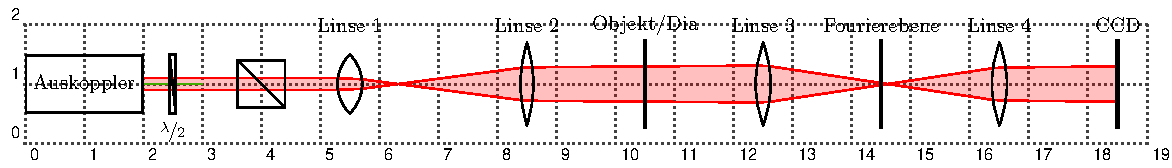
\includegraphics[width=1\linewidth]{graphs/versuchsaufbau/4f-aufbau.pdf}
	\caption[Schematische Skizze des 4f-Aufbaus]{
		Schematische Skizze des 4f-Aufbaus. Der Laserstrahl passiert nach Verlassen des Auskopplers eine $\nicefrac{\lambda}{2}$-Platte und anschließend einen Strahlteiler. Der zweite Teil des Strahls, welcher vom Strahlteiler abgelenkt wird, trifft auf eine Strahlblockierung und wird nicht weiter verwendet. Zwischen Linse 2 und 3 befindet sich die Halterung für das Objekt/Dia, in der Fourierebene wird entweder eine zweite Kamera oder ein Filter positioniert. Die CCD Kamera am Ende des Strahlengangs befindet sich in der Abbildungsebene des Aufbaus.
	}
	\label{fig:4f-aufbau}
\end{figure}

In diesem sogenannten 4f-Aufbau passierte der Laserstrahl nach der Reflektion am ersten Spiegel eine $\nicefrac{\lambda}{2}$-Platte und dahinter einen Strahlteiler. Mit Hilfe des Strahlteilers wurde eine eindeutige Polarisierung sicher gestellt, während mit dem Plättchen die Lichtmenge der durchlässigen Polarisation eingestellt werden konnte.\\

Um die abzubildenden Objekte vollständig ausleuchten zu können, wurde der Laserstrahl in diesem Aufbau mit Hilfe der ersten beiden Linsen aufgeweitet und wieder kollimiert. Im Brennpunkt der dritten Linse befand sich ein Objektträger in der Gegenstandsebene. In diesem wurden die abzubildenden Objekte angebracht. Die Fourierebene befindet sich im Brennpunkt der Linsen 3 und 4. Nach der vierten Linse wird der Strahl erneut kollimiert und trifft auf die CCD Kamera, Kamera 1. Hier wird das Objekt möglichst originalgetreu abgebildet. Um Aufnahmen der Fourierspektren zu erhalten, wurde bei Bedarf eine zweite Kamera, Kamera 2, in der Fourierebene montiert. \\ 

Verwendet wurden hierbei Linsen der Brennweiten wie folgt: Linse 1 mit $f_{1}=\unit[20]{mm}$, Linse 2 mit $f_{2}=\unit[200]{mm}$, Linse 3 und 4 mit $f_{3}=f_{4}=\unit[100]{mm}$. Direkt hinter der Auskopplung wurde zusätzlich ein Spiegel, optimiert für Wellenlängen von \unit[400-700]{nm}, in den 4f-Aufbau aufgenommen, um den Verlauf des Laserstrahls im optischen Pfad besser feinjustieren zu können. Leider wurde die Strahlqualität durch diesen stark beeinträchtigt, so dass zusätzlich ein Pinhole zwischen Linse 1 und 2 notwendig war, um eine gaußähnliche Strahlmode zu erhalten.\\


\begin{figure}[h]
	\centering
	\includegraphicsRS[width=0.7\linewidth][.7]{images/4f-anfang.JPG}
	\caption[Vorderer Teil des 4f-Aufbaus]{
		Vorderer Teil des realisierten 4f-Aufbaus. \textbf{Hintere Reihe, von links nach rechts:} Faserauskoppler; Strahlblockade für den im Strahlteiler reflektierten Anteil. \textbf{Vordere Reihe, von links nach rechts:} zusätzlich eingebauter Spiegel; $\nicefrac{\lambda}{2}$-Platte; Strahlteiler; Diahalter; Linse 1; Pinhole, welches am rechten Bildrand hinter Linse 1 zu sehen ist.
	}
	\label{fig:_DSC7961}
\end{figure}

\begin{figure}[ht]
	\centering
	\includegraphicsRS[width=0.43\linewidth][.45]{images/_DSC7988.JPG}~
	\includegraphicsRS[width=0.43\linewidth][.45]{images/IMG_2223.jpg}
	%\vspace{2cm}\hspace{2cm}
	\caption[Mode vor und nach Verwendung eines Pinholes]{
		\textbf{Links:} Mode des Laserstrahls am Ende des optischen Pfades vor Einbau des Pinholes.\\
		\textbf{Rechts:} Mode des Laserstrahls am Ende des optischen Pfades nach Einbau des Pinholes.
	}
	\label{fig:_DSC7988}
\end{figure}


Als Hilfsmittel bei der Justage des 4f-Aufbaus wurde hier eine Iris verwendet. Mit dieser konnte beispielsweise die Kollimierung des Laserstrahls hinter Linse 2 Überprüft werden, indem die Öffnung der Iris auf die Strahlbreite eingestellt wurde und anschließend entlang des optischen Pfades verschoben wurde. Dabei konnte überprüft werden, ob die Breite des Laserstrahls konstant blieb. Die Justage der Linse konnte somit verbessert werden. Außerdem ließ sich mit Hilfe der Iris über die gleiche Vorgehensweise die Höhe des Strahls entlang des gesamten 4f-Aufbaus kontrollieren und diese dann mit Hilfe der Technik des Walkens optimieren. 


\begin{comment}
\begin{figure}
	\centering
	\includegraphicsRS[width=0.7\linewidth, angle=90]{images/_DSC7967.JPG}
	\caption{Foto des hier realisierten 4f-Aufbaus.}
	\label{fig:_DSC7967}
\end{figure}
\end{comment}

\clearpage


